
\PassOptionsToPackage{table}{xcolor}

\documentclass{gaiasocbeamer}


\usepackage{pgf,tikz}
\usetikzlibrary{calc}
\usepackage{movie15}

%
% Empty frame environment: useful for page-filling images.
%
% argument is frame title
%
\newenvironment{emptyframe}[1]{%
\begin{frame}[plain]
  \hypertarget<1>{#1}{}
  \only<1>{\pdfbookmark[2]{#1}{#1}}}%
{\end{frame}}



% ----------------------


%\usepackage{pdfpages}

\author[William O'Mullane]{William O'Mullane }

\date[05/03/2017]{ 5$^{\text{th}}$ March  2017, LSST JTM, \\ LA, California, USA. }


\institute[LSST]{Data Management\\LSST}
% ----------------------


\AtBeginSection[]  % "Beamer, do the following at the start of every section"
{
\begin{frame}<beamer>
\addtocounter{framenumber}{-1}
\frametitle{Outline} % make a frame titled "Outline"
\tableofcontents[currentsection]  % show TOC and highlight current section
\end{frame}
}


\AtBeginSubsection[]
{
   \begin{frame}
\addtocounter{framenumber}{-1}
       \frametitle{Outline}
       \tableofcontents[currentsection,currentsubsection]
   \end{frame}
}


%
% Empty frame environment: useful for page-filling images.
%
% argument is frame title
%
\newenvironment{emptyframe}[1]{%
\begin{frame}[plain]
  \hypertarget<1>{#1}{}
  \only<1>{\pdfbookmark[2]{#1}{#1}}}%
{\end{frame}}




\title[Gaia GBU]{Building the Gaia ground segment\ {\small revisited }}


\date[10/01/2017]{ January 10$^{\text{th}}$  2017, LSST Tucson}


% ----------------------


\begin{document}
\frame{\titlepage}
\frame{\frametitle{what did and did not work ..} 
\begin{center}
Or \\
\huge
{\color{green}the good} \\
{\color{red} the bad} \\
and \\
{\color{blue}the ugly}.
\end{center}
\normalsize
The western is quintessentially  American, that one was Italian though and it was shot in Spain.

}

\section{Initial Set up}

%
%%%%%%%%%%%%%%%%%%%%%%%%%%%%%%%%%%%%%%%%%%%%%%%%%%%%%%%%%%%%%%%%%%%%%%%%%%%%%
%
% Gaia Data Processing and Analysis Consortium
%
%%%%%%%%%%%%%%%%%%%%%%%%%%%%%%%%%%%%%%%%%%%%%%%%%%%%%%%%%%%%%%%%%%%%%%%%%%%%%
%
\begin{emptyframe}{Gaia Data Processing and Analysis Consortium}
  \vskip-3.3mm
  \begin{tikzpicture}
    \node (map) at (0,0) [anchor=south west]
    {\hspace{-2.75cm}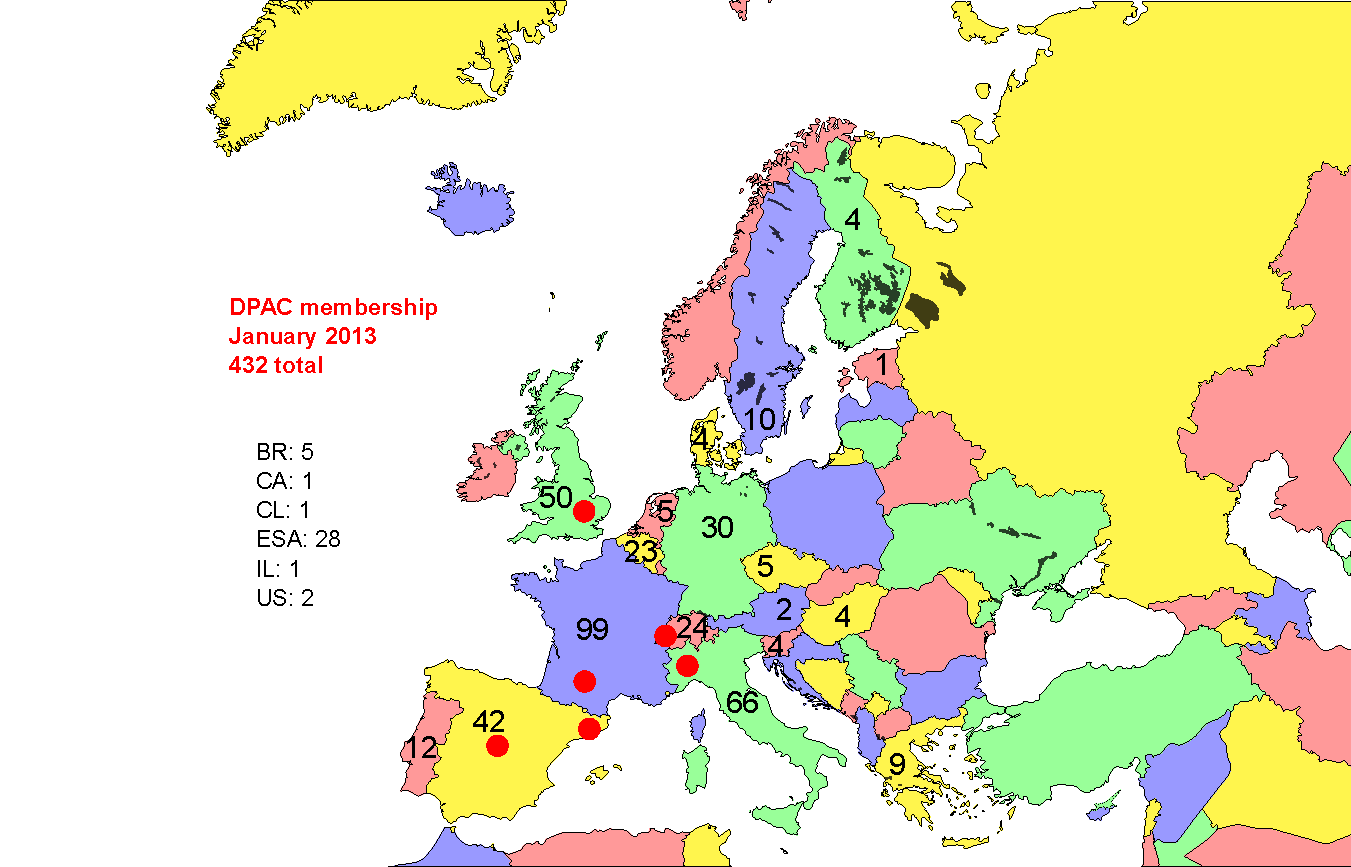
\includegraphics[height=\paperheight]{images/DpacMembershipMapAndDPCs.pdf}};
    \node at ($(map.north west)+(4,-1.7)$)
    {
\includegraphics[height=1.3cm]{images/dpac_logo.pdf}};
    \node at ($(map.north east)-(0.1,0.5)$) [anchor=north east, text width=4.8cm, text badly ragged,
    fill=white, fill opacity=0.8, text opacity=1, rounded corners=5pt]
    {\begin{itemize}
      \item Gaia data processing is a Pan-European cooperation
        \begin{itemize}
          \item Over 1000 staff years effort since 2006
          \item Processing power spread over 6 centres
          \item Supported through national funding
          \item Additional support from EC Marie Curie and ESF
        \end{itemize}
    \end{itemize}
  };
  \node at ($(map.south east)+(-0.3,0.3)$) [anchor=south
  east]{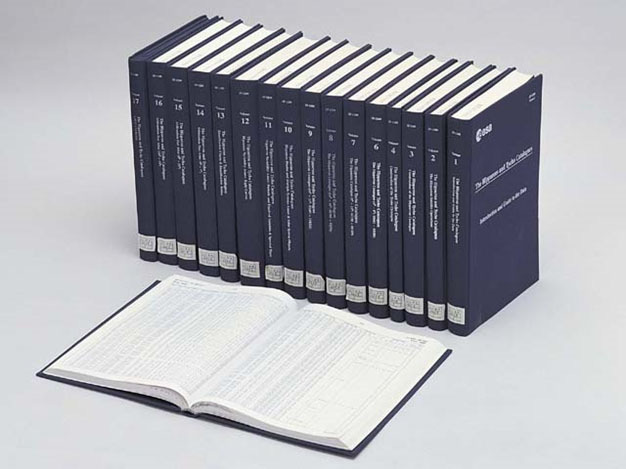
\includegraphics[height=3cm]{images/catalogue_hipparcos.pdf}};
\end{tikzpicture}
\end{emptyframe}


\frame {\frametitle{  In the beginning} 
\begin{itemize}
  \item initial ideas for ground segment were in place for the study in 2000 \citell{LL:ESA-SCI(2000)4}
  \item already clear then we would have distributed processing in multiple centres (though not mentioned)
  \item Intention was to have autonomy between coordination units
\pause
  \item Interviewed several project leaders for \cite{LL:WOM-003} in 2004/5 --- tried to learn from
    them \ldots
    \begin{itemize}
      \item Included LSST (Kantor) 
  \item Management came out as the most difficult part of all projects \ldots so I will leave that until last.
    \end{itemize}
  \item some things started before DPAC --- simulations and GIS studies for example.
  \item Finally DPAC is large --- I am sure you can find someone in DPAC to disagree with anything I say. 
\end{itemize}
}


\section{Standards and Tools}

\frame {\frametitle{  Language (spoken) and conventions } 
\begin{itemize}
  \item Very important in large groups
  \item Which way is up on Gaia, which is a row and column on focal plane, which quaternion to use
  \item {\color{green} dealt with quite early on in \citell{LL:BAS-003}}
    \begin{itemize}
      \item still Astrium have a different definition for $X,Y,Z$ on Gaia
      \item at least in the consortium there is only one  --- could have been much worse  
    \end{itemize}
    \pause
  \item What is a product, a Work Package --- why is 10 months $=$ 1 year
  \item also dealt with early on in \citell{LL:WOM-001}
    \pause
  \item Then there are Acronyms \url{http://gaia.esac.esa.int/gpdb/glossary.txt} and an acronym tool
    for TeX files (e.g. Appendix \ref{sect:acr})
    \pause
  \item having a complete engineering guideline early was good \citell{LL:JH-001}
\end{itemize}
}


\frame {\frametitle{ Parameters and data models } 
\begin{itemize}
%\item Which value do we use for speed of light, measurements of Gaia instrument 
  \item Avoid different values of constants in peoples code \ldots 
  \item The Gaia Parameter Database was set up early on for this \citep{2005ESASP.576...67D}
    \begin{itemize}
      \item all constants in one place; web searchable configuration controlled (Only updated by Jos De Bruijne)
      \item published as constants for Java (can also do C, Fortran\ldots) so you may refer to a particular version
    \end{itemize}
  \item then the actual data model --- what exactly is an AstroElementary?
    \begin{itemize}
      \item entire data model defined in multi-user dictionary tool; includes Units on each field.
        \begin{itemize}
          \item good for astronomers --- computer people find it harder to handle 
        \end{itemize}
      \item from it we generate data instance classes and schemas for storage.
      \item {\color{green} ONLY data model not processing} --- all objects are dumb
%	\item This was in UML (Rose) in the 90s but it was impractical to continue..
    \end{itemize}
  \item {\color{green} These are logical extensions of having agreed conventions\ldots}
\end{itemize}
}

\frame {
  \frametitle{  Flight Operations Procedures in MOC}
\vspace{-0.5cm}
\begin{center}	
   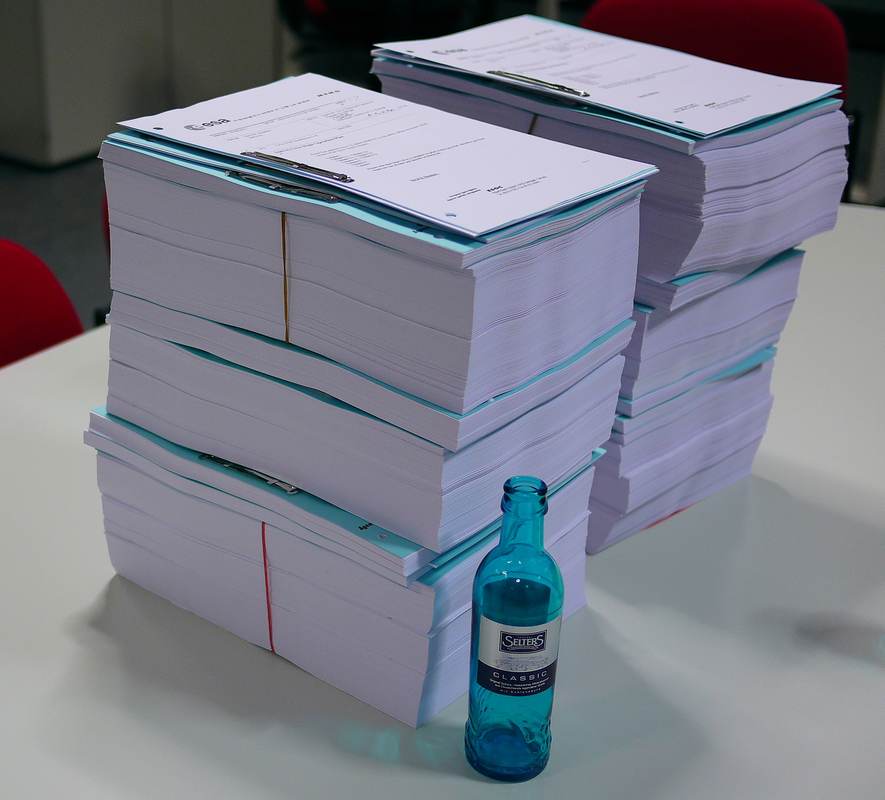
\includegraphics[width=0.6\textwidth,trim=0cm 0cm 0cm 0cm]{images/fops}

\end{center}
The FOP is followed by the spacecraft operators - the paper copy is just in case the computers fail.
	We should try to keep documentation useful.
}

\frame {\frametitle{ Have a standard: DPAC follows ECSS }
\begin{columns}
  \begin{column}{0.5\textwidth}
%\pgfputat{\pgfxy(0,0)}{\pgfbox[left,top]{
    %\begin{center}
      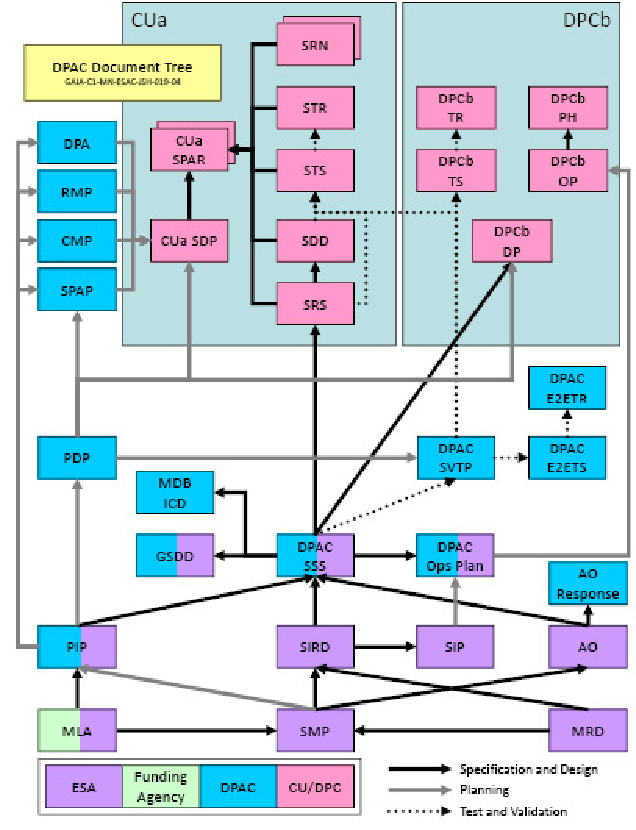
\includegraphics[width=0.9\textwidth]{images/doctree-crop}\\
    %\end{center}
      {\tiny Doctree by  John Hoar \citellp{LL:RD-010}}\hfill
%}}
  \end{column}
  \begin{column}{0.5\textwidth}
    \vskip-7.3cm
    \textbf{European Cooperation for Space Standardization}
    \begin{itemize}
      \item ECSS tailored as in figure
        \begin{itemize}
          \item LaTeX Templates/examples provided (by SOC) 
          \item Documents are iterated ---  All of this is done for all DPAC products.
          \item {\color{green} It is very good to have a standard set of documents augmented by technical notes and streamlined ECSS}
          \item Some still found it too heavy --- other reports requested beyond the standard ones.
        \end{itemize}
      \item DPAC had sufficient QA people ($\sim1/$CU) from the start to help with this% and create examples and templates.
    \end{itemize}
  \end{column}
\end{columns}
}

\frame {\frametitle{  Software licensing } 
\begin{itemize}
  \item protect intellectual property  --- grant use to the consortium 
  \item often forgotten or not well dealt with -  or worse ignored!
  \item DPAC in general agree to LGPL \citellp{LL:WOM-019} -  some institutes e.g. ESA, do not allow staff to write GPL code.
  \item Being allowed LGPL in ESA for Gaia involved lawyers and directors and some of my time and some Herschel people. 
    \begin{itemize}
  	\item now ALL ESA science missions can use LGPL with D/SRE approval.
    \end{itemize}
\end{itemize}
\begin{center}
      
\includegraphics[width=0.7\textwidth]{images/dilbertsl}\\
{\tiny You may use up to seven (7) cartoons per year at no costs as part of our fair use policy.}
\end{center}
}



\frame {\frametitle{ Single Sign on  Gaia Portal } 
\begin{itemize}
  \item \url{http://www.rssd.esa.int/index.php?project=MYPORTAL&page=index} hosted at ESTEC; set up
    eons ago\ldots
  \item Names, emails and affiliations (phone numbers, photo, address) of all Gaia people
  \item Single login (LDAP) for 
    \begin{itemize}
      \item Livelink --- for all published documents
      \item Wiki --- for wiki things (meeting setup etc.); always draft nearly always out of date
      \item Mantis --- for all issues 
    \end{itemize}
  \item Same LDAP for SVN, MDB dictionary etc
  \item Single sign on is perhaps not great but having one LDAP for authentication of everything
    is fabulous!
  \item {\color{blue} Having information in SVN, Livelink and possibly on a wiki is not great but we
  do not have a solution}
  \item {\color{green} Having single agreed set of collaboration tools from the outset excellent.}
\end{itemize}
}

\frame{\frametitle{Development tools}
\begin{itemize}
  \item All DPAC code and docs in Subversion, hosted at ESAC 
    \begin{itemize}
      \item Access control according to Group membership in the LDAP 
    \end{itemize}
  \item Mantis for centralized issue tracking (includes risks and actions)
    \begin{itemize}
      \item ALL DPAC issues in one system hosted at ESTEC 
      \item {\color{red} Jira would probably be better }
  \end{itemize}
\pause
  \item{\color{green} Having one language is good \citep{2011arXiv1108.0355O}} agreed 2006

    \citellp{LL:JH-001} --- only one verification part is NOT in Java. 
    \begin{itemize}
      \item Can have a library of standard  routines  GaiaTools (Relativity, Field Angle Calculator,
        Ephemeris handling\ldots)
        \begin{itemize}
          \item {\color{red} The set of routines were not defined hence GaiaTools is a bit of
          hodgepodge mess\ldots}
          \item {\color{blue} Counter argument for common tools is (unnecessary)
          interdependence\ldots}
        \end{itemize}
      \item all libs in Nexus 
      \item builds with Ant; {\color{red} Maven might be the thing to use now}
      \item automated builds with Hudson/Jenkins (previously cruisecontrol)
      \item {\color{blue} virtual machines make some reasons for Java invalid}
    \end{itemize}
\end{itemize}
}


\section{Management}
\frame {\frametitle{  Communication } 
\begin{itemize}
  \item Internal 
    \begin{itemize}
      \item the newsletter is excellent and well contributed to
      \item (few) focused working groups and working meetings 
      \item To date never had a consortium meeting; {\color{red} probably a mistake.} --- we do intend
        this during processing
      \item As for any project cost of entry for new people is very high {\color{blue} --- no obvious
      solution }
    \end{itemize}
\pause
  \item ESA policy initially to reduce contact between DPAC and Astrium (who construct Gaia)
    {\color{red} not good}
\pause
  \item External 
    \begin{itemize}
      \item perhaps could have had a better DPAC website 
      \item ESA PR also not great (ok as they point out they have a tiny fraction of NASA budget)
      \item LSST.org is very nice.
      \item {\color{blue}Publication policy was dealt with very late }
    \end{itemize}
\end{itemize}
}

\frame {\frametitle{  Operations Rehearsals } 
\begin{itemize}
  \item Have had 4 operations rehearsals in the last 2 years
  \item Not tests as such; intended for training staff and checking procedures 
  \item Move the teams mind-set away from just development and towards building a usable system.
  \item Helped find defects as well as other needs (missing features and functions) in the  software
    running at DPCs.
  \item These are good {\color{blue} could have started earlier }
  \item {\color{red} It became clear operational awareness was low across DPAC, i.e.\ in terms of
  turn around of commanding to Gaia and how it works, how data flows, general constraints of
satellite operations}
\end{itemize}
}


\frame {\frametitle{  Requirements Management } 
\begin{itemize}
  \item Some requirements at an appropriate level are very useful. 
    \begin{itemize}
        {\color{red}
      \item could have been better formulated
    \item separation of performance, software, and science requirements should have been clearer}
  \end{itemize}
\item DPAC stayed away from requirements tools like DOORS though
\item Used macros in LaTeX for requirements and scripts to build trace tables
\item All requirements and test reports then ingested in the Information Management Tool \citellp{2012SPIE.8449E..0GC}
\item {\color{red} Could probably have put more effort in this earlier}
  \begin{itemize}
    \item might then have decided to start up some CUs later.
  \end{itemize}
\item Reviews are an unavoidable part of all this 
  \begin{itemize}
    \item ESA reviews are {\color{blue} too formal and too large}
    \item External reviewers like Innocente (\citell{LL:VI-001},\citell{LL:VI-002}) {\color{green}
    very good} --- would be good to have a few external review {\em partners}
  \end{itemize}
\end{itemize}
}


\frame[allowframebreaks] {\frametitle{  Management and  science } 
All large projects, and especially science projects, have management {\em issues}
\begin{itemize}
  \item In 2006 we had a big management training week for the DPAC management --- though sceptical
    to start most found it good
  \item Science project management is a little different but still books like
    \citep{handy1993understanding} are quite useful
  \item Cyclic (Agile type) development seems well suited to science
    \begin{itemize}
      \item we chose six month cycles --- probably too long 
      \item {\color{green} some prototypes started real early} \citep{1999BaltA...8...57O}
      \item we have great simulations --- they started in 1998 before Gaia was accepted
        \begin{itemize}
          \item Still they always seemed to be a little behind what people wanted --- {\color{blue} we
          have no solution for that, could not start earlier}
          \item simulator fell out of the ECSS rigour --- testing etc\ldots
        \end{itemize}
      \item we did a lot of testing; {\color{blue} some tests were probably not appropriate in hindsight}
      \item {\color{red} despite aiming for test driven development --- NOT ENOUGH effort in
      testing and many systems only recently got continuous integration}
    \end{itemize}
  \item Scientific institutes are not good at managing things like software projects (hard anyway)
    \begin{itemize}
      \item {\color{red} Interface control between software was insufficient } --- data model was
        not enough
      \item Perhaps ESA should have taken control of all critical software 
      \item ESA is stepping back from this type of role in future missions and was not
        totally happy about the level of involvement of ESAC in DPAC.
    \end{itemize}
  \item Note: industrial contracts for scientific software are difficult
    \begin{itemize}
	\item but science consortia neeed managers and engineers earlier 
      \item Did an experiment with this on Gaia very early on
      \item XMM have there own woeful tale to tell
      \item Still CNES have been {\em stuck}  with this model --- even worse as we drive the project
        quite dynamically.
    \end{itemize}
\end{itemize}
}


\frame {
  \frametitle{  DPAC Executive  in 2011  at ULB}
\vspace{-0.5cm}
\begin{center}	
   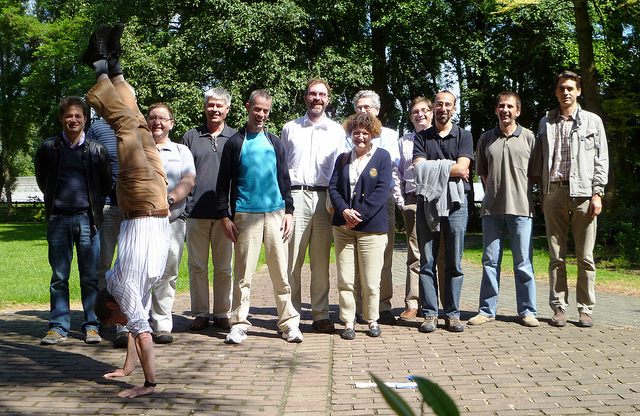
\includegraphics[width=0.9\textwidth,trim=0cm 0cm 0cm 0cm]{images/dpace13h}

At ULB Belgium	 - yes we will stand on our hands if we need to.\\
	DPACE is small and technically focused. Meeting about twice  a year.
	
\end{center}
}

\frame[allowframebreaks]{\frametitle{  DPAC Management } 
\begin{itemize}
  \item Started out with the idea of limited number (9) of decoupled Coordination Units(CU) ---
    {\color{green} Good}
    \begin{itemize}
      \item this resulted from much discussion in the DACC --- {\color{green} It was good to have
      dedicated group to decide how the consortium was set up; n.b.\ DACC$\ne$DPACE} 
    \item {\color{green} Having relatively small executive (DPACE) being technically focused was
    also good}
  \item All in DPACE may not have agreed with all decisions but ALL backed them once made 
\end{itemize}
\item Data processing centres added under CUs --- also a bit decoupled --- {\color{blue} Could have been
more coupled and better controlled}
  \begin{itemize}
    \item DPCs often started too late 
      \begin{itemize}
        \item led to a lack of {\em engineering} in many areas ---
          {\color{red} lack of software engineers in initial phases, many hires were
        astronomers }
        \item performance aspects of the systems were handled too late
        \item integration efforts were underestimated 
      \end{itemize}
    \item CUs turned out not to be so decoupled in software, e.g.\ data models need to be the
      same\ldots
    \item May have been a mistake to allow different frameworks/DBMSs in different DPCs
      \begin{itemize}
        \item certainly inefficient in effort terms 
        \item however it is too easy to make things NOT work --- I  did not want to {\em force}
          everyone down the route I followed
      \end{itemize}
  \end{itemize}
\item despite starting with a management course --- Management support was insufficient 
  \begin{itemize}
    \item More management support in setting up the CUs and reporting would have been good ---
      {\color{red} perhaps more emphasis should have been put here by DPACE}
    \item The Project Office (PO) came along too late to assist with shaping this --- it was good and should have started earlier 
  \end{itemize}
\item Too collaborative? 
  \begin{itemize}
    \item DPAC was broadly inclusive --- CU leaders on paper had the chance to include or not groups
      and WPs but in fact no one was left out
    \item this has lead to some inefficiencies --- perhaps we could be smaller and more focused 
    \item we possibly should have jettisoned some work packages, groups, and individuals early on
    \item {\color{blue} In a proper phased approach some CUs could probably have started 2 years
    later with minimum presence at kick off} 
  \end{itemize}
\item Too flexible and too inflexible 
  \begin{itemize}
    \item there are many configuration control boards and other groups to manage change
    \item no one wants any change to anything --- {\em until the moment they want a change  then it
      should be immediate}
    \item {\color{red} We have found no solution to this} 
  \end{itemize}
\item {\color{blue}In hindsight some work packages were misplaced}
\end{itemize}
}


\section{Conclusion}

\frame{\frametitle{  Conclusion } 
\begin{columns}
\column{0.33\textwidth}
\pgfputat{\pgfxy(0,0)}{\pgfbox[left,top]{
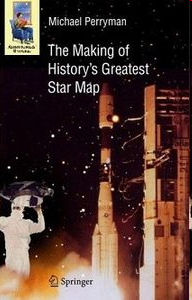
\includegraphics[scale=0.8,trim=0cm 0cm 0pt 0pt]{images/starmap}
}}
\cite{Perryman2010}
\column{0.67\textwidth}
\vspace{-15pt}
\begin{itemize}
  \item many of us dreamed of a Gaia Processing Institute - only a dream for
    us; but for LSST !!
\pause
  \item Much mentioned here is contentious --- others do not see it exactly as I do.
  \item For me DPAC started of well largely due to strong initial leadership especially
    from Perryman
  \item All agree we are fortunate to have some excellent people in DPAC 
\pause
  \item thanks to DPACE for their input to this presentation and to DPAC for all their work over the past years.
  \item How this all works out will soon be seen\ldots probably a tough year ahead !
\end{itemize}

\end{columns}
}





\section{Management of Gaia}
\frame {\frametitle{  Communication } 
\begin{itemize}
  \item Internal communication: 
    \begin{itemize}
      \item Some say could have been better.
      \item Few focused working groups and working meetings.
      \item As for any project cost of entry for new people is very high {\color{blue} --- no obvious solution}.
    \end{itemize}
  \item ESA policy initially to reduce contact between DPAC and Astrium (who construct Gaia)
    {\color{red} not good}.
  \item External communication: 
    \begin{itemize}
      \item Perhaps could have had a better DPAC website.
      \item ESA PR also not great (ok as they point out they have a tiny fraction of NASA budget).
      \item {\color{blue}Publication policy was dealt with very late.}
    \end{itemize}
\end{itemize}
}


\frame {\frametitle{  Requirements Management } 
\begin{itemize}
  \item Some requirements at an appropriate level are very useful. 
    \begin{itemize}
        {\color{red}
      \item Many could have been better formulated.
    \item Separation of performance, software, and science requirements should have been clearer.}
  \end{itemize}
\item All requirements and test reports then ingested in the Information Management Tool \citep{2012SPIE.8449E..0GC}:
    \begin{itemize}
\item Automated testing provided much requirements verification.
\item Operations Rehearsals used to validate many requirements.
\item {\color{red} Could probably have put more effort in this earlier.}
  \end{itemize}
\item Cumbersome ESA Reviews are an unavoidable part of all this:
    \begin{itemize}
	\item  {\color{red}Just do it.}  - that means many expected documents ..
	\item  {\color{blue} Had to convince all collaborators to also support reviews.} 
	\item {\color{green} Projected cohesive unified team image }
	\item  on LSST  believe you have no choice in this - less formal reviews which is probably worse for you perhaps better for LSST goals
  \end{itemize}
\end{itemize}
}


\frame[allowframebreaks] {\frametitle{  Management and  science } 
All large projects, and especially science projects, have management {\em issues}.
\begin{itemize}
  \item In 2006 we had a big management training week for the DPAC management --- though sceptical
    to start most found it good:
	\begin{itemize}
	\item Despite this management support was still lacking.
        \end{itemize}
  \item Science project management is a little different, still books like
    \citep{handy1993understanding} are quite useful.
  \item Cyclic (Agile type) development seems well suited to science:
    \begin{itemize}
      \item We chose six month cycles --- probably too long (good for reporting).
      \item {\color{green} Some prototypes started very early} \citep{1999BaltA...8...57O}.
      \item  We have great simulations --- {\color{green}they started in 1998 }before Gaia was accepted:
        \begin{itemize}
          \item Still they always seemed to be a little behind what people wanted --- {\color{blue} we
          have no solution for that, could not start earlier.}
          \item Simulator fell out of the ECSS rigour --- testing etc\ldots
        \end{itemize}
      \item We did a lot of testing; {\color{blue} some tests were probably not appropriate in hindsight}.
      \item {\color{red} Despite aiming for test driven development --- NOT ENOUGH effort in
      testing and many systems only recently got continuous integration.}
    \end{itemize}
  \item Scientific institutes are not good at managing things like software projects (hard anyway):
    \begin{itemize}
      \item {\color{red} Interface control between software was insufficient } --- data model was not enough. {\color{red} perceive this in LSST now and Datamodel is not as rigorous}
      \item Perhaps ESA should have taken control of all critical software.
      \item ESA is stepping back from this type of role in future missions and was not
        totally happy about the level of involvement of ESAC in DPAC.
    \end{itemize}
  \item Industrial contracts for scientific software are very difficult:
    \begin{itemize}
      \item Did an experiment with this on Gaia very early on.
      \item XMM have their own woeful tale to tell.
	\item Science consortia need managers and engineers already in the early phases
    \begin{itemize}
	
        \item  Noted lack of {\em engineering} in many areas ---
          {\color{red} lack of software engineers in initial phases, many hires were astronomers}.
    \end{itemize}

    \end{itemize}



\item DPAC too collaborative? 
  \begin{itemize}
    \item DPAC was broadly inclusive --- CU leaders on paper had the chance to include or not groups
      and WPs but in fact no one was left out.
    \item This has lead to some inefficiencies --- perhaps we could be smaller and more focused.
    \item We possibly should have jettisoned some work packages, groups, and individuals early on.
    \item {\color{blue} In a proper phased approach some CUs could probably have started 2 years
    later with minimum presence at kick off} 
  \end{itemize}
\item Too flexible and too inflexible:
  \begin{itemize}
    \item There are many configuration control boards and other groups to manage change.
    \item {\color{blue}No one wants any change to anything --- {\em until the moment they want a change  then it
      should be immediate!}}
    \item {\color{red} We have found no solution to this.} 
  \end{itemize}
\end{itemize}
}






\frame {
  \frametitle{ The END }
\begin{itemize}
\item Looking forward to working with a great set of people in DM and LSST
\item LSST has  potential for huge impact in Astronomy
\item I will use my experience and training to help get DM delivered  
\item I also have a lot to learn from LSST people so I hope you will all help me - intend to visit all the DM sites soon
\item I have an open door policy, extended to phone email in DM ! (I do close my door when in a telecon)
\item Looking forward to the first LSST images !
\end{itemize}
\begin{center}	
\huge{\color{red} Questions ??}
\end{center}	

}



 \appendix
\section {Acronyms}\label{sect:acr}

\frame[allowframebreaks]{\frametitle{Acronyms}
\tiny
The following table has been generated from the on-line Gaia acronym list:
\newline\newline%decrement table counter so table sin doc start at 1.
\addtocounter{table}{-1}
\begin{longtable}{|l|p{0.8\textwidth}|}\hline 
\textbf{Acronym} & \textbf{Description}  \\\hline
API&Application Programming Interface \\\hline
CU&Coordination Unit (in DPAC) \\\hline
DM&Data Management (LSST) \\\hline
DPAC&Data Processing and Analysis Consortium \\\hline
DPACE&Data Processing and Analysis Consortium Executive \\\hline
ECSS&European Cooperation for Space Standardisation \\\hline
ESA&European Space Agency \\\hline
ESAC&European Space Astronomy Centre (VilSpa) \\\hline
ESF&European Science Foundation \\\hline
ESTEC&European Space research and TEchnology Centre (ESA) \\\hline
FOP&Flight Operation Procedure (Plan) \\\hline
GIS&(Astrometric) Global Iterative Solution \\\hline
IOA&Institute of Astronomy (Cambridge; also denoted IOA) \\\hline
LDAP&Lightweight Directory Access Protocol \\\hline
LSST&Large Synoptic Surrvey Telescope \\\hline
LTD&LSST the Docs \\\hline
LaTeX&(Leslie) Lamport TeX (document markup language and document preparation system) \\\hline
MDB&Main Database \\\hline
MOC&Mission Operations Centre \\\hline
NASA&National Aeronautics and Space Administration (USA) \\\hline
PR&Progress Report \\\hline
QA&Quality Assurance \\\hline
SDSS&Sloan Digital Sky Survey \\\hline
SOC&Science Operations Centre \\\hline
SVN&SubVersioN \\\hline
TOC&Table of Contents \\\hline
USA&United States of America \\\hline
WP&Work Package \\\hline
XMM&X-ray Multi-mirror Mission (ESA; officially known as XMM-Newton) \\\hline
\end{longtable} 

}

\section {References}\label{sect:ref}
\frame[allowframebreaks]{\frametitle{ References }
\tiny
\bibliographystyle{gaia_aa}
\bibliography{gaia_livelink_valid,gaia_refs,gaia_books,gaia_refs_ads}
\normalsize

}
\end{document}
